\section{Configuracao dos Experimentos}
Este capitulo apresenta os resultados obtidos para o Gerador R-MAT
e o Kernel 2 do Graph500,  a busca em largura (BFS). 
A metrica principal de comparacao e TEPS (\textit{Traversed Edges Per Second}), discutida no capitulo 
sobre o Graph500, e o tempo de execucao em segundos. O valor usado como 
referencia e a mediana de TEPS de todas as buscas realizadas,
pois o benchmark executa varias buscas a partir de raizes diferentes.

Os experimentos foram organizados em dois ambientes. O primeiro e o computador
pessoal usado no desenvolvimento, com processador Ryzen 5 5600x, 32 GB de memoria
RAM e uma GPU NVIDIA RTX 5060 Ti com 16 GB de memoria. O segundo e um ambiente
GB200 com uma CPU e quatro GPUs. 

As execucoes disponiveis foram realizadas com fator de arestas igual a 16, 64
buscas BFS. Neste trabalho, esses resultados sao
considerados validos para a analise de desempenho.

\section{Implementacoes Comparadas}
Tres implementacoes sao consideradas na comparacao:

\begin{itemize}
\item \textbf{MPI CPU referencia}: implementacao de referencia do Graph500,
executada apenas na CPU com processos MPI. Foi utilizado 12 worker 1 worker por thread.
\item \textbf{NVSHMEM hibrida CPU/GPU}: implementacao em que a GPU expande a
fronteira e emite operacoes NVSHMEM, mas a CPU ainda participa da coordenacao
global entre niveis, incluindo sincronizacoes e reducoes. Foi utilizado somente 1 worker.
\item \textbf{NVSHMEM GPU exclusiva}: implementacao em que a BFS e coordenada
em GPU, com comunicacao NVSHMEM iniciada pelo dispositivo e sem usar a CPU como
participante recorrente entre os niveis da busca. Foi utilizado somente 1 worker.
\end{itemize}

\section{Resultados no Computador Pessoal}
No computador pessoal, a maior escala disponivel no conjunto de resultados foi 
\texttt{SCALE=22}. 

\begin{table}[H]
\centering
\resizebox{\textwidth}{!}{
\begin{tabular}{l|c|c|c}
\hline
Implementacao           & SCALE & Gerador R-MAT (s) & Mediana TEPS \(H\) \\
\hline
MPI CPU referencia      & 22    & 3,57838  & $1{,}95437 \times 10^{8}$ \\
NVSHMEM hibrida CPU/GPU & 22    & 0,483327 & $2{,}53907 \times 10^{8}$ \\
NVSHMEM GPU exclusiva   & --    & -- & -- \\
\hline
\end{tabular}
}
\caption{Resultados no computador pessoal na maior escala disponivel (22).}
\label{tab:resultados-pc}
\end{table}

A Figura~\ref{fig:teps-por-escala} mostra a mediana de TEPS por escala para os
resultados disponiveis. 

\begin{figure}[H]
\centering
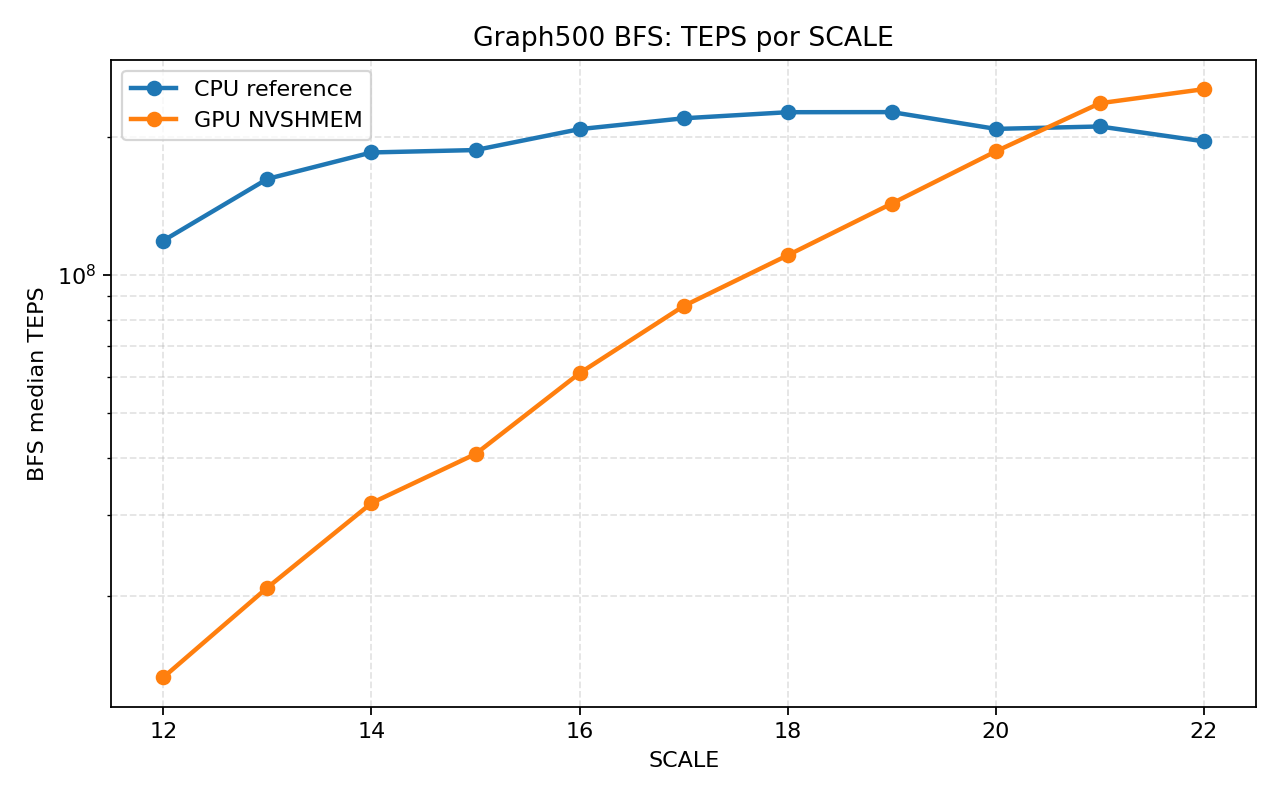
\includegraphics[width=\textwidth]{results/cpu_gpu_bfs_20260701_230022/teps_by_scale.png}
\caption{Mediana de TEPS por escala no computador pessoal.}
\label{fig:teps-por-escala}
\end{figure}

O grafico evidencia que a implementacao de referencia
em CPU apresenta melhor desempenho nas escalas pequenas e medias, enquanto a
implementacao CUDA/NVSHMEM cresce de forma mais acentuada com o tamanho do grafo.
Na mediana de TEPS, a GPU tambem passa a superar a CPU a partir de \texttt{SCALE=21}.

\section{Resultados no GB200}
TODO
